\documentclass{article}
\usepackage[utf8]{inputenc} %кодировка
\usepackage[T2A]{fontenc}
\usepackage[english,russian]{babel} %русификатор 
\usepackage{mathtools} %библиотека матеши
\usepackage[left=1cm,right=1cm,top=2cm,bottom=2cm,bindingoffset=0cm]{geometry} %изменение отступов на листе
\usepackage{amsmath}
\usepackage{graphicx} %библиотека для графики и картинок
\graphicspath{}
\DeclareGraphicsExtensions{.pdf,.png,.jpg}
\usepackage{subcaption}
\usepackage{pgfplots}
\usepackage{array}
\usepackage{pgfplots}
\pgfplotsset{compat=1.16}

\begin{document}
% НАЧАЛО ТИТУЛЬНОГО ЛИСТА
\begin{center}
    \Large
    Федеральное государственное автономное \\
    образовательное учреждение высшего образования \\ 
    «Национальный исследовательский университет ИТМО»\\
    \vspace{0.5cm}
    \large
    Факультет программной инженерии и компьютерной техники \\
    Направление подготовки 09.03.04 Программная инженерия \\
    \vspace{1cm}
    \Large
    \textbf{Отчёт по лабораторной работе №2} \\
    По дисциплине «Математическая статистика» (четвёртый семестр)\\
    Построение оценки параметров законов распределения и оценки функции распределения и плотности вероятности.\\
    \large
    \vspace{8cm}

    \begin{minipage}{.33\textwidth}
    \end{minipage}
    \hfill
    \begin{minipage}{.4\textwidth}
    
        \textbf{Студент}: \vspace{.1cm} \\
        \ Билошицкий Михаи Владимирович\\
        \ Беляев Михаил Сергеевич\\
        \ Сиразетдинов Азат Ниязович\\
        \textbf{Преподаватель}:  \\
        \ Милованович Екатерина Воиславовна
    \end{minipage}
    \vfill
Санкт-Петербург\\ 2024 г.
\end{center}
\thispagestyle{empty}

% КОНЕЦ ТИТУЛЬНОГО ЛИСТА 
\newpage
\section*{Цель работы}
Цель данной работы состоит в том, чтобы на основании опытных данных, используя метод моментов, построить оценки параметров законов распределения и оценки функции респределения и плотности вероятности.
\section*{Данные }
Закон: равномерный закон распределения\\
Выборка: -2.53, -0.74, -4.49, 1.27, -5.37, 3.77, -3.35, -1.87, -2.62, -0.38
\section{Вариационный ряд}
-5.37, -4.49, -3.35, -2.62, -2.53, -1.87, -0.74, -0.38, 1.27, 3.77
\section{Точечная оценка математического ожидания}
\[\overline{m} = \frac{1}{n}\sum_{i=1}^{n}x_i \approx -1.63\]
\[\overline{\sigma}^2 = \frac{1}{n-1}\sum_{i=1}^{n}(x_i-\overline{m})^2 \approx 7.43\]
\section{Построение оценки}
Используя метод метод моментов, построим оценки параметров нормального закона распределения, где нормальный закон распределения имеет следующий вид:
\\ \\
Функция плотности случайной величины:
\[f(x) = \frac{1}{\sqrt{2 \pi \sigma}} e^{- \frac{(x-m)^2}{2 \sigma^2}}\]
Функция распределения:
\[\quad F(x) = \frac{1}{2} \left[1 + \Phi\left(\frac{x-m}{\sigma}\right)\right]\]
\[\text{где } \Phi(z) - \text{функция Лапласа. }\]
\[\Phi(z) = \frac{2}{\sqrt{2\pi}} \int\limits_0^z e^{-\frac{t^2}{2}} dt.\]

\section{Метод моментов}

Выразим числовые параметры теоретического распределения через моменты распределения, оценненные по выборки. 
\\ \\
Неизвестных параметров в нормальном законе распределения нет, кроме тех, что можно посчитать из выборки, а именно математического ожидания, дисперсии и стандартного отклонения. Вычислим:
\\ \\
Математическое ожидание:
\[\overline{m} = \frac{1}{n}\sum_{i=1}^{n}x_i \approx -1.63\]
Дисперсия:
\[\overline{\sigma}^2 = \frac{1}{n-1}\sum_{i=1}^{n}(x_i-\overline{m})^2 \approx 7.43\]
Стандартное отклонение:
\[\overline{\sigma} = \sqrt{\overline{\sigma}^2} \approx 2.73 \]
Подставим $m, \sigma^2, \sigma:$
\[f(x) = \frac{1}{\sqrt{2 \pi \cdot 2.73}} e^{- \frac{(x - (-1.63))^2}{2 \cdot 7.43}};\]
\[\quad F(x) = \frac{1}{2} \left[1 + \Phi\left(\frac{x - (-1.63)}{2.73}\right)\right],\]
Упростим и получим результат:

\[f(x) = \frac{1}{\sqrt{2 \pi \cdot 2.73}} e^{- \frac{(x + 1.63)^2}{2 \cdot 7.43}}\]
\[\quad F(x) = \frac{1}{2} \left[1 + \Phi\left(\frac{x + 1.63}{2.73}\right)\right]\]
\[\text{где } \Phi(z) - \text{функция Лапласа. }\]
\[\Phi(z) = \frac{2}{\sqrt{2\pi}} \int\limits_0^z e^{-\frac{t^2}{2}} dt.\]

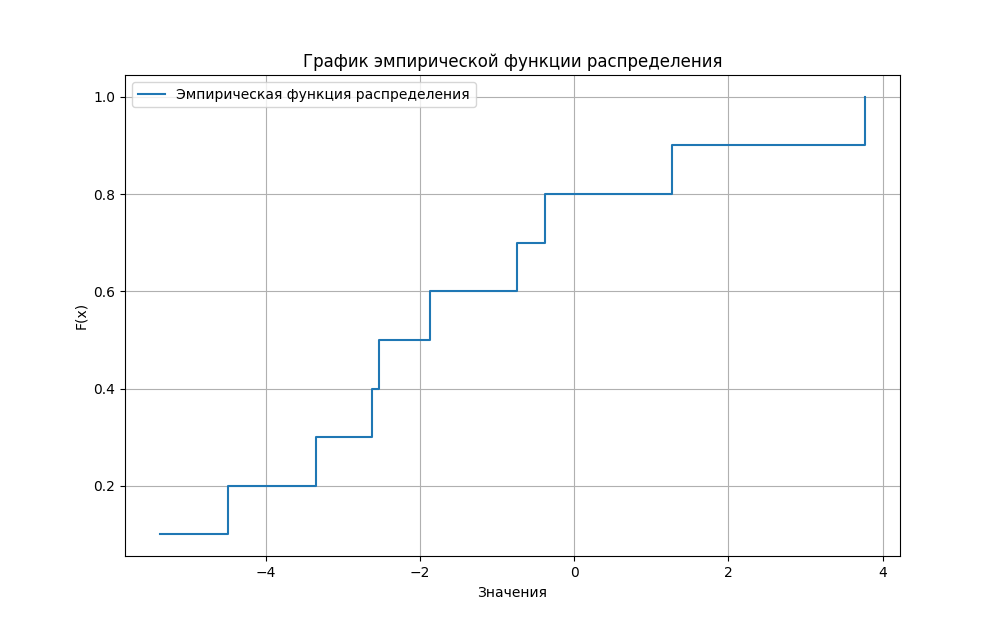
\includegraphics[width=.9\textwidth]{emp.png}

\newpage
\section{Построение оценок}
Построение графика плотности случайной величины и графика функции распределения:\\

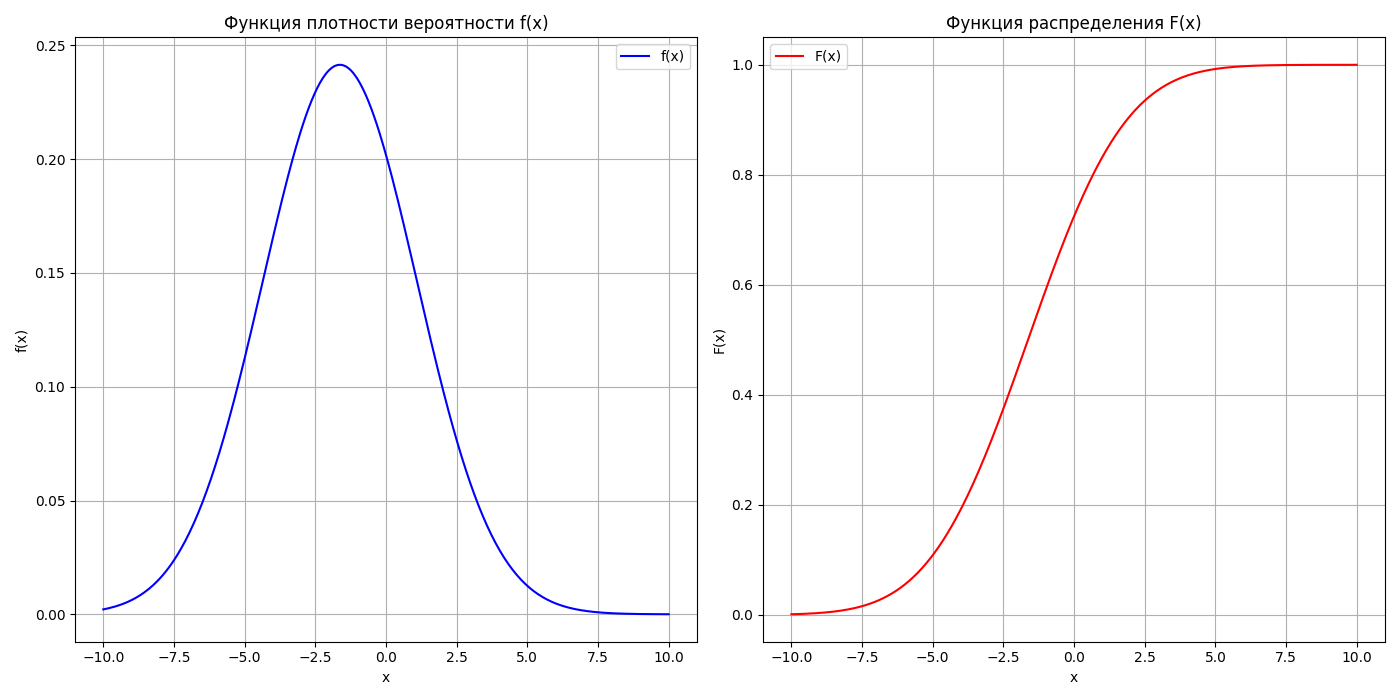
\includegraphics[width=0.9\textwidth]{funcs.png}

\section*{Вывод}
На основании опытных данных нашли при помощи метода моментов параметры равномерного закона распределения, а также построили функцию распределения и плотность вероятности.
\end{document}
\includegraphics[width=.9\textwidth]{123}